\chapter{Foam-Like Cells and Relaxation}

\section{Space Divided Among Seeds}

A third kind of cellular structure divides space instead of filling it. Given a set of points, assign every location to the nearest point. The set of locations assigned to one point is its cell, the cells are convex polygons in the plane, and together they tile it. The tiling is the Voronoi diagram of the points. It describes, to a first approximation, the cells of a dry foam, the territories of animals that defend the ground nearest their nests, the catchments of wells, and the plan of a market in which each customer visits the nearest stall. In each case the points are the primary data and the cells are a derived structure, so the useful questions concern what the cells inherit from the points. This chapter asks what a random arrangement of points produces, how an iterative rule that moves each point towards the centre of its own cell changes the arrangement, and what can be measured to say so.

To avoid edge effects, all arrangements are placed on a torus, the unit square with opposite sides identified, and computed by tiling nine copies of the points and keeping the cells of the central copy. The cells of the central copy are polygons that may extend past the square, and together they cover it exactly once. The code is in \texttt{foam.py}. It uses SciPy's \texttt{Voronoi}, orders each cell's vertices by angle about its point, and counts a side wherever consecutive vertices are distinct. The generator is NumPy's \texttt{default\_rng}, and the same seed gave the same points and the same side counts on repetition.

\section{Two Identities That Hold for Every Arrangement}

Two properties were checked on five random arrangements of $400$ points before any statistics were taken. The cell areas summed to $1$, to the twelve decimals printed, so that the cells tile the torus with neither gap nor overlap. The mean number of sides was $6$ exactly, in every arrangement. The second property is an instance of Euler's formula. On a torus a polygonal tiling has $V-E+F=0$, and when three cells meet at every vertex, as happens with probability one for random points, each vertex has three edges, so $2E=3V$ and the average cell has $2E/F=6$ sides. The identity says nothing about the points, and it holds for the regular hexagonal tiling and for the most irregular one alike. It follows that the mean number of sides cannot distinguish arrangements, and the quantities that can are the spread of the side counts and the spread of the cell areas.

\section{Random Points and Relaxed Points}

The relaxation rule, usually attributed to Lloyd, moves every point to the centroid of its cell and recomputes the cells. One application is one step. The rule does not change the number of points, and it is deterministic once the starting points are fixed, so an arrangement is a function of the seed and the number of steps. The statistics below are means over $20$ seeds of $400$ points each, with the standard deviation across seeds after each $\pm$. The side-count spread is the standard deviation of the number of sides within one arrangement, the hexagon fraction is the share of cells with exactly six sides, and the area spread is the standard deviation of cell area divided by its mean.

\begin{center}
\begin{tabular}{rrrrr}
\toprule
Steps & Mean sides & Side-count spread & Hexagon fraction & Area spread\\
\midrule
0  & $6.000\pm0.000$ & $1.346\pm0.040$ & $0.287\pm0.021$ & $0.522\pm0.033$\\
1  & $6.000\pm0.000$ & $1.069\pm0.041$ & $0.376\pm0.024$ & $0.373\pm0.028$\\
2  & $6.000\pm0.000$ & $0.945\pm0.025$ & $0.418\pm0.025$ & $0.303\pm0.026$\\
5  & $6.000\pm0.000$ & $0.811\pm0.021$ & $0.481\pm0.032$ & $0.212\pm0.024$\\
10 & $6.000\pm0.000$ & $0.718\pm0.028$ & $0.550\pm0.027$ & $0.157\pm0.021$\\
20 & $6.000\pm0.000$ & $0.628\pm0.025$ & $0.623\pm0.026$ & $0.114\pm0.018$\\
50 & $6.000\pm0.000$ & $0.544\pm0.019$ & $0.705\pm0.022$ & $0.074\pm0.009$\\
\bottomrule
\end{tabular}
\end{center}

The first step does the most work: the area spread falls from $0.522$ to $0.373$. After that the improvement slows. The area spread falls by about a third between steps $20$ and $50$, and the side-count spread falls by about a seventh. Even after $50$ steps, $29.5\%$ of the cells are not hexagons, so the arrangement has not become a regular lattice, and the departures from six sides persist. In the relaxed Blender example of Section 18.5 the non-hexagons are almost all five-sided or seven-sided, $36$ and $32$ of $150$ cells. Whether the hexagon fraction would approach one with many more steps was not tested, and the table gives no reason to assume that it does.

For the random arrangement the spread of the side counts, $1.346$, corresponds to a variance of $1.81$, and the area spread, $0.522$, can be compared with the values recalled, and not rechecked, from the literature on random Voronoi tessellations of about $1.78$ and $0.53$. The agreement is within the seed-to-seed scatter, and the literature values are recalled and were not checked against a source.

\section{Large Cells Have More Sides}

In dry foams larger cells tend to have more sides, a relation named for Lewis that is usually stated as a linear dependence of mean area on the number of sides. The relation was measured on the random arrangements, pooling $8000$ cells from the $20$ seeds, with each cell's area divided by its arrangement's mean area.

\begin{center}
\begin{tabular}{rrrrrrrrr}
\toprule
Sides & 3 & 4 & 5 & 6 & 7 & 8 & 9 & 10\\
\midrule
Cells & 84 & 905 & 2052 & 2299 & 1631 & 691 & 266 & 60\\
Mean relative area & 0.384 & 0.561 & 0.780 & 0.997 & 1.210 & 1.450 & 1.700 & 1.856\\
\bottomrule
\end{tabular}
\end{center}

A straight line fitted to the means for $4$ to $8$ sides has slope $0.219$ per side and reaches zero area at $1.45$ sides, so the dependence is close to linear over that range, with the six-sided cell very close to average. The slope at the ends departs a little: from $3$ to $4$ sides the area rises by $0.177$, and from $9$ to $10$ by $0.156$, against $0.219$ in the middle. The measurement shows a monotone, nearly linear increase for these arrangements. It does not test the relation as a law of foams, because a random point set is not a foam, and it does not settle why the relation holds. After relaxation the cells have nearly equal areas, so the relation weakens as the arrangement approaches a regular one, and that was not measured.

\section{Cells in Blender}

All cells of an arrangement are placed in Blender as one mesh with one polygon per cell. The number of sides is stored as an integer attribute on each face, and one material reads that attribute with an Attribute node of the geometry type and maps it from $4$ to $8$ through a blue--white--red ramp, so the whole arrangement uses one object, one mesh and one material. This differs from the preceding chapters, where the quantity of interest was stored on each object, and the choice here follows from the structure: the cells belong together as one tiling, and sharing one mesh preserves their adjacency. The script is \texttt{foam\_blender.py}.

For $150$ points from seed $2$, before and after $20$ relaxation steps, the mesh held $150$ polygons in each case, and the polygon areas summed to $1.000000$, which is the area of the torus, so the mesh tiles the square exactly as the calculation did. The mean number of sides read from the stored attribute was $6.0000$ in both cases. The attribute equalled the number of vertices of each polygon for every cell. The histogram of side counts for $3$ through $10$ sides was $1,15,43,45,24,16,4,2$ for the random points and $0,0,36,80,32,2,0,0$ after relaxation, so the relaxed arrangement has no cell with fewer than five or more than eight sides. The relaxed points were regenerated from the seed and the step count and were identical. Under $20$ steps the points moved on average by $0.044$ of the side of the square, which is about half of the mean spacing of about $0.082$ for $150$ points.

\begin{figure}[ht]
\centering
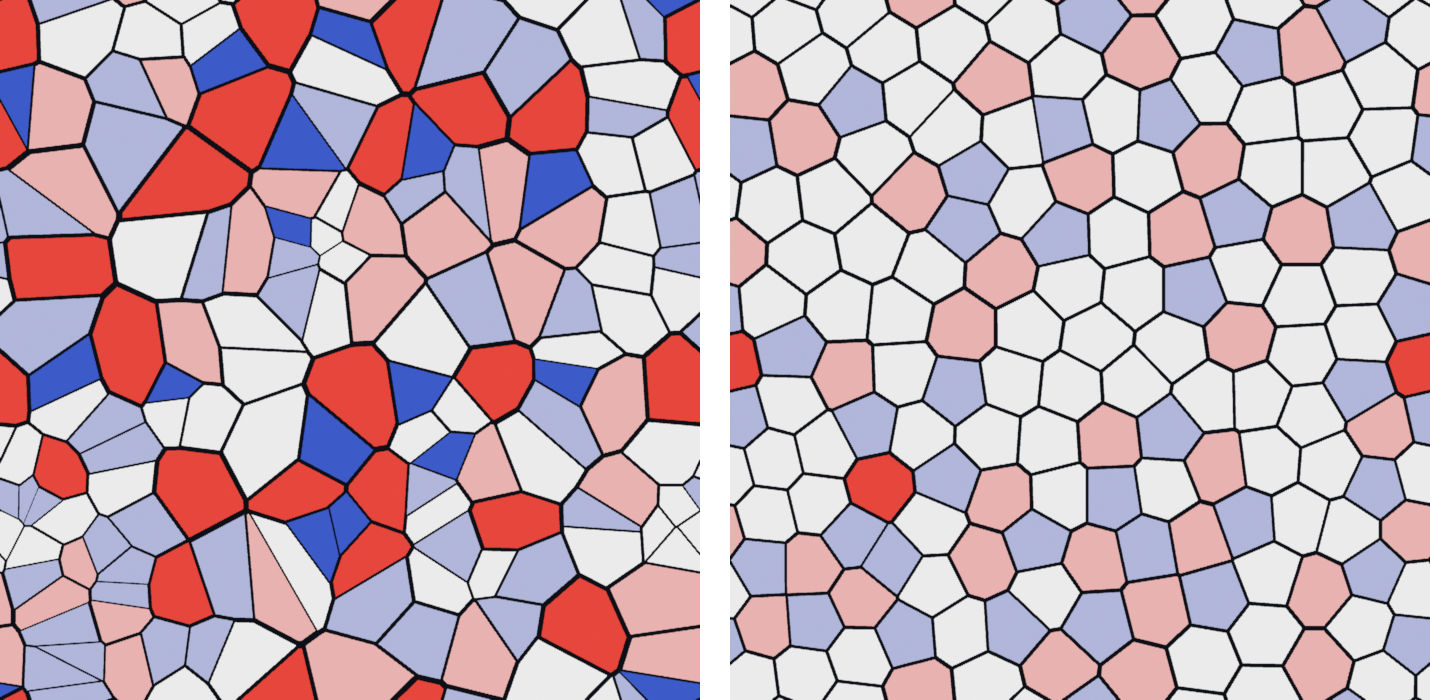
\includegraphics[width=\textwidth]{figs/fig18_foam.png}
\caption{The unit torus tiled by $150$ cells coloured by number of sides, from four (blue) through six (white) to eight (red), with one material reading a face attribute. Left, random points, seed $2$. Right, the same points after $20$ relaxation steps. The panels were rendered separately from the same mesh construction, with the cells drawn at $0.94$ of their size so that the walls are visible. Thin cells at left are real cells of the random arrangement, and the area sum confirms that the tiling is complete.}
\end{figure}

\section{What These Experiments Do Not Show}

All results are for points on a torus, with $400$ points in the tables and $150$ in the Blender scene, and with $20$ seeds for the statistics, so edge effects, which dominate small real foams, were excluded by construction. The relaxation rule was stopped at $50$ steps, and nothing was measured about its limit. The side-count and area spreads for random points are compared with literature values that are recalled from reading. The linear relation of area to number of sides was observed over a pooled sample and not tested for other densities or for relaxed arrangements. Nothing here shows that a real foam, a territory pattern or a market follows the Voronoi rule, which assigns each location to the nearest point and ignores the surface tension, the competition and the travel costs that govern the real systems. The experiments show what a nearest-point rule does with random and relaxed points, with the precision stated.

\begin{exercise}[18.1: Many more steps]
Run the relaxation for $200$ and $1000$ steps on $10$ seeds of $400$ points, report the hexagon fraction at each, and say whether the table's trend continues. State what a stable fraction below one would mean for the structure.
\end{exercise}

\begin{exercise}[18.2: Density]
Repeat the random-points statistics at $100$, $400$ and $1600$ points, and report whether the side-count spread and area spread depend on the number of points. State what you expect before running it.
\end{exercise}

\begin{exercise}[18.3: A different seed process]
Replace the uniform random points by points placed with a minimum separation (a hard-core process) and compare the side-count spread and area spread with the random case and with the relaxed case at the same number of cells. Describe where the hard-core arrangement falls between them.
\end{exercise}

\begin{exercise}[18.4: Walls as edges]
Extract the shared edges of one relaxed arrangement from the mesh, count them, and check the relation $2E=3V$ implied in Section 18.2. Report any vertex at which four cells meet and the tolerance you used to decide.
\end{exercise}
